\documentclass[leqno, openany]{memoir}
\setulmarginsandblock{3.5cm}{3.5cm}{*}
\setlrmarginsandblock{3cm}{3.5cm}{*}
\checkandfixthelayout

\usepackage{amsmath}
\usepackage{amssymb}
\usepackage{amsthm}
%\usepackage{MnSymbol}
\usepackage{bm}
\usepackage{accents}
\usepackage{mathtools}
\usepackage{tikz}
\usetikzlibrary{calc}
\usetikzlibrary{automata,positioning}
\usepackage{tikz-cd}
\usepackage{forest}
\usepackage{braket} 
\usepackage{listings}
\usepackage{mdframed}
\usepackage{verbatim}
\usepackage{physics}
%\usepackage{/home/patrickl/homework/macaulay2}

%font
\usepackage[osf]{mathpazo}
\usepackage{microtype}

%CS packages
\usepackage{algorithmicx}
\usepackage{algpseudocode}
\usepackage{algorithm}

% typeset and bib
\usepackage[english]{babel} 
\usepackage[utf8]{inputenc} 
\usepackage[backend=biber, style=alphabetic]{biblatex}
\usepackage[bookmarks, colorlinks, breaklinks]{hyperref} 
\hypersetup{linkcolor=black,citecolor=black,filecolor=black,urlcolor=black}

% other formatting packages
\usepackage{float}
\usepackage{booktabs}
\usepackage{enumitem}
\usepackage{csquotes}
\usepackage{titlesec}
\usepackage{titling}
\usepackage{fancyhdr}
\usepackage{lastpage}
\usepackage{parskip}

\usepackage{lipsum}

% delimiters
\DeclarePairedDelimiter{\gen}{\langle}{\rangle}
\DeclarePairedDelimiter{\floor}{\lfloor}{\rfloor}
\DeclarePairedDelimiter{\ceil}{\lceil}{\rceil}


\newtheorem{thm}{Theorem}[section]
\newtheorem{cor}[thm]{Corollary}
\newtheorem{prop}[thm]{Proposition}
\newtheorem{lem}[thm]{Lemma}
\newtheorem{conj}[thm]{Conjecture}
\newtheorem{quest}[thm]{Question}

\theoremstyle{definition}
\newtheorem{defn}[thm]{Definition}
\newtheorem{defns}[thm]{Definitions}
\newtheorem{con}[thm]{Construction}
\newtheorem{exm}[thm]{Example}
\newtheorem{exms}[thm]{Examples}
\newtheorem{notn}[thm]{Notation}
\newtheorem{notns}[thm]{Notations}
\newtheorem{addm}[thm]{Addendum}
\newtheorem{exer}[thm]{Exercise}

\theoremstyle{remark}
\newtheorem{rmk}[thm]{Remark}
\newtheorem{rmks}[thm]{Remarks}
\newtheorem{warn}[thm]{Warning}
\newtheorem{sch}[thm]{Scholium}


% unnumbered theorems
\theoremstyle{plain}
\newtheorem*{thm*}{Theorem}
\newtheorem*{prop*}{Proposition}
\newtheorem*{lem*}{Lemma}
\newtheorem*{cor*}{Corollary}
\newtheorem*{conj*}{Conjecture}

% unnumbered definitions
\theoremstyle{definition}
\newtheorem*{defn*}{Definition}
\newtheorem*{exer*}{Exercise}
\newtheorem*{defns*}{Definitions}
\newtheorem*{con*}{Construction}
\newtheorem*{exm*}{Example}
\newtheorem*{exms*}{Examples}
\newtheorem*{notn*}{Notation}
\newtheorem*{notns*}{Notations}
\newtheorem*{addm*}{Addendum}


\theoremstyle{remark}
\newtheorem*{rmk*}{Remark}

% shortcuts
\newcommand{\Ima}{\mathrm{Im}}
\newcommand{\A}{\mathbb{A}}
\newcommand{\N}{\mathbb{N}}
\newcommand{\R}{\mathbb{R}}
\newcommand{\C}{\mathbb{C}}
\newcommand{\Z}{\mathbb{Z}}
\newcommand{\Q}{\mathbb{Q}}
\renewcommand{\k}{\Bbbk}
\renewcommand{\P}{\mathbb{P}}
\newcommand{\M}{\overline{M}}
\newcommand{\g}{\mathfrak{g}}
\newcommand{\h}{\mathfrak{h}}
\newcommand{\n}{\mathfrak{n}}
\renewcommand{\b}{\mathfrak{b}}
\newcommand{\ep}{\varepsilon}
\newcommand*{\dt}[1]{%
   \accentset{\mbox{\Huge\bfseries .}}{#1}}
\renewcommand{\abstractname}{Official Description}
\newcommand{\mc}[1]{\mathcal{#1}}
\newcommand{\T}{\mathbb{T}}
\newcommand{\mf}[1]{\mathfrak{#1}}
\newcommand{\mr}[1]{\mathrm{#1}}
\newcommand{\ms}[1]{\mathsf{#1}}
\newcommand{\ol}[1]{\overline{#1}}
\newcommand{\wt}[1]{\widetilde{#1}}

\DeclareMathOperator{\Der}{Der}
\DeclareMathOperator{\Hom}{Hom}
\DeclareMathOperator{\End}{End}
\DeclareMathOperator{\ad}{ad}
\DeclareMathOperator{\Aut}{Aut}
\DeclareMathOperator{\Rad}{Rad}
\DeclareMathOperator{\supp}{supp}
\DeclareMathOperator{\sgn}{sgn}
\DeclareMathOperator{\spec}{Spec}

% Section formatting
\titleformat{\section}
    {\Large\sffamily\scshape\bfseries}{\thesection}{1em}{}
\titleformat{\subsection}[runin]
    {\large\sffamily\bfseries}{\thesubsection}{1em}{}
\titleformat{\subsubsection}[runin]{\normalfont\itshape}{\thesubsubsection}{1em}{}

\title{COURSE TITLE}
\author{Lectures by INSTRUCTOR, Notes by NOTETAKER}
\date{SEMESTER}

\newcommand*{\titleSW}
    {\begingroup% Story of Writing
    \raggedleft
    \vspace*{\baselineskip}
    {\Huge\itshape Algebraic Topology \\ Fall 2020}\\[\baselineskip]
    {\large\itshape Notes by Patrick Lei}\\[0.2\textheight]
    {\Large Lectures by Mohammed Abouzaid}\par
    \vfill
    {\Large \sffamily Columbia University}
    \vspace*{\baselineskip}
\endgroup}
\pagestyle{simple}

\chapterstyle{ell}


%\renewcommand{\cftchapterpagefont}{}
\renewcommand\cftchapterfont{\sffamily}
\renewcommand\cftsectionfont{\scshape}
\renewcommand*{\cftchapterleader}{}
\renewcommand*{\cftsectionleader}{}
\renewcommand*{\cftsubsectionleader}{}
\renewcommand*{\cftchapterformatpnum}[1]{~\textbullet~#1}
\renewcommand*{\cftsectionformatpnum}[1]{~\textbullet~#1}
\renewcommand*{\cftsubsectionformatpnum}[1]{~\textbullet~#1}
\renewcommand{\cftchapterafterpnum}{\cftparfillskip}
\renewcommand{\cftsectionafterpnum}{\cftparfillskip}
\renewcommand{\cftsubsectionafterpnum}{\cftparfillskip}
\setrmarg{3.55em plus 1fil}
\setsecnumdepth{subsection}
\maxsecnumdepth{subsection}
\settocdepth{subsection}

\begin{document}
    
\begin{titlingpage}
\titleSW
\end{titlingpage}

\thispagestyle{empty}
\section*{Disclaimer}%
\label{sec:disclaimer}

These notes were taken during lecture using the \texttt{vimtex} package of the editor \texttt{neovim}. 
Any errors are mine and not the instructor's. 
In addition, my notes are picture-free (but will include commutative diagrams) and are a mix of my mathematical style and that of the instructor.
If you find any errors, please contact me at \texttt{plei@math.columbia.edu}.
\newpage


\tableofcontents

\chapter{Basics of Homotopy Theory}%
\label{cha:basic_notions}

\section{Categorical Notions}%
\label{sec:categorical_notions}

We will use the book \textit{Algebraic Topology} by Tammo tom Dieck. We will use categorical language, even if we don't strictly need it. We will denote the category of (Hausdorff) topological spaces and continuous maps by $\ms{Top}$. There are two ways of thinking about algebraic topology:
\begin{enumerate}
    \item Extracting algebraic invariants from spaces;
    \item Doing algebra with spaces.
\end{enumerate}

Homotopy is an equivalence relation on $\ms{Top}(X,Y)$. 

\begin{defn}
    A \textit{homotopy} from $f$ to $g$ is a map $H: X \times I \to Y$ such that $H \circ i_0 = f$ and $H \circ i_1 = g$. Intuitively, this is a way to interpolate between $f$ and $g$. Alternatively, a homotopy is a path in $Y^X$ with the compact-open topology.
\end{defn} 

To show that homotopy is an equivalence relation, it is easy to show that $f$ is self-homotopic. To see that homotopy is symmetric, we can simply reverse the interval. Finally, to see that homotopy is transitive, we can just perform each homotopy twice as fast and then concatenate.

\begin{defn}
The \textit{homotopy category} $\ms{hTop}$ is the category whose objects are spaces and whose morphisms are homotopy classes of maps. We need to check that composition preserves the notion of homotopy.
\end{defn}

Now denote the \textit{category of based spaces} by $\ms{Top}^*$, where a based space is a space $X$ with a map $* \to X$. The corresponding homotopy category is denoted by $\ms{hTop}^*$. Here, the homotopy is required to fix the basepoint.

\begin{rmk}
    The transition from spaces to based spaces is like upgrading from semigroups to monoids.
\end{rmk}

\begin{rmk}
    There is a functor 
    \begin{align*}
        \ms{Top} \to \ms{Top}^* \\
        X \mapsto (X \sqcup \{*\}, *).
    \end{align*}
\end{rmk}

\begin{exm}
    It is easy to see that $\ms{Top}(*,X) \cong X$. Similarly, $\ms{Top}^*(S^0,(X,*)) \cong X$. Then, we can see that $\ms{hTop}(*,X) \cong \ms{hTop}(S^0,X)$ is the set of path components of $X$.
\end{exm}

\section{Fundamental Group and Groupoid}%
\label{sec:fundamental_group_and_groupoid}

\begin{exm}
    We will now consider morphisms from the circle. The set $\ms{Top}(S^1,X)$ is the free loop space $\mc{L}X$. In the based case, we get the \textit{based loop space} $\Omega X$. Then $\ms{hTop}(S^1,X)$ is the path components of $\mc{L}X$, and similarly, $hTop^*(S^1,X) \cong \pi_1(X,*)$, where $\pi_1$ is the fundamental group.
\end{exm}

It should be surprising that $[S^1,X]$ is a group. In fact, it is independent on the path component of $*$ up to inner automorphism. However, we can distinguish a class of isomorphisms up to conjugation. The identity of this group is the constant path at the basepoint. Next, we need to consider the product in the group. This is simply concatenation, which is given by the (cogroup) operation $S^1 \to S^1 \vee S^1$. Because the two components of the wedge cannot be swapped by a homotopy, this operation is not commutative.

Next, we need to check that this is compatible with homotopy. Then the operation on homotopy classes is the product in $\pi_1$. To check associativity, we can check that the total operation of pinching at $1/3$ and pinching at $2/3$ commutes.

Finally, the inverse of a path $g$ is simply $t \mapsto g(1-t)$. To construct an isomorphism between $\pi_1(X,*_1)$ and $\pi_1(X, *_2)$, choose a path $g$ between the two basepoints and then send $f \mapsto g^{-1} f g$.

We will now discuss an unbased analogue of the fundamental group. Beginning with the path space $\mathsf{Top}([0,1],X)$, we can consider the evaluations at $0$ and $1$. Then over $(x,y)$, can consider homotopy classes of maps with fixed endpoints to obtain the set $\Pi X(x,y)$.

\begin{prop}
    $\Pi X(x,y)$ are the morphisms of a \textit{groupoid} with objects $X$.
\end{prop}

\begin{rmk}
    $\Pi X(x,x) \cong \pi_1(X,x)$. The fundamental group is much nicer, but is hard to compute because it depends on the basepoint.
\end{rmk}

\begin{defn}
    A \textit{homotopy equivalence} $f:X \to Y$ is a map that induces an isomorphism in the homotopy category. 
\end{defn}

\begin{prop}
    A homotopy equivalence $X \to Y$ induces an equivalence of categories $\Pi f: \Pi X \to \Pi Y$. Recall here that an equivalence of categories is a fully faithful and essentially surjective functor. Equivalently, it is a functor has an inverse up to natural isomorphism.
\end{prop}

\begin{proof}
    The homotopy defines a natural transformation from $\mr{id}_X$ to $\Pi gf$. Let $g$ be a homotopy inverse, and $H$ be a homotopy and let $H$ be a homotopy from $\mr{id}_X$ to $gf$. We can evaluate $H$ on the path $\gamma$, and this gives a homotopy between $x \to y \to g(f(y))$ and $x \to g(f(x)) \to g(f(y))$. Therefore, we have equality up to homotopy, so this gives a natural transformation. Because we are working in a groupoid, this is automatically an isomorphism.
\end{proof}

\begin{cor}
    Homotopy equivalences induce isomorphisms of fundamental groups.
\end{cor}

Suppose we have a diagram of the form
\begin{equation}
\begin{tikzcd}
    A \arrow{r}{f_1} \arrow{d}{f_2} & B_1 \\
    B_2
\end{tikzcd}.
\end{equation}
Then a \textit{pushout} $C$ is the colimit of this diagram. This means that there exist maps $g_1, g_2$ such that
\begin{equation}
\begin{tikzcd}
    A \arrow{r}{f_1} \arrow{d}{f_2} & B_1 \arrow{d}{g_1} \\
    B_2 \arrow{r}{g_2} & C
\end{tikzcd}
\end{equation}
commutes and $(C, g_1, g_2)$ is universal: For any $X$ and commutative diagram, there exists a unique map such that
\begin{equation}
\begin{tikzcd}
    A \arrow{r}{f_1} \arrow{d}{f_2} & B_1 \arrow{d}{g_1} \arrow{ddr} & \\
    B_2 \arrow{r}{g_2} \arrow{drr} & C \arrow[dashrightarrow]{dr} &  \\
                                   & & X
\end{tikzcd}
\end{equation}
commutes.

\begin{thm}[Seifert-van Kampen Theorem]
    Let $X$ be a topological space and $X_0, X_1$ subspaes whose interiors cover $X$. Then set $X_{01} = X_0 \cap X_1$. Then 
\begin{equation}
\begin{tikzcd}
    \Pi X_{01} \arrow{r} \arrow{d} & \Pi X_0 \arrow{d} \\
    \Pi X_1 \arrow{r} & \Pi X
\end{tikzcd}
\end{equation}
is a pushout diagram of groupoids.
\end{thm}

\begin{proof}
    Consider a groupoid $G$ and commutative diagram
\begin{equation}
\begin{tikzcd}
    \Pi X_{01} \arrow{r}{f_0} \arrow{d}{f_1} & \Pi X_0 \arrow{d}{h_0} \\
    \Pi X_1 \arrow{r}{h_1} & G
\end{tikzcd}.
\end{equation}
We will construct $\Pi X \xrightarrow{h} G$. Then we need to write $h(x)$ as an object of $G$. If $x \in X_1$, set $h(x) = h_1(x)$, and if $x \in X_0$, set $h(x) = h_0(x)$. Because (1.5) commutes, this is well-defined. Now we define $h$ on the level of morphisms. Subdivide paths so that all segments lie in either $X_0$ or $X_1$. Then on each such segment, the diagram specifies $h(\gamma_i)$, and define $h(\gamma) = h(\gamma_0) h(\gamma_1) \cdots h(\gamma_n)$.

Finally, we need to prove that this definition is independent of the choice of representative of homotopy class. We can subdivide the homotopy so each equare lies in either $X_0$ or $X_1$, and then $h_1, h_1$ are well-defined, so $h$ is independent of the homotopy class.
\end{proof}

\begin{exm}
    We can use Seifert-van Kampen to compute the fundamental group of $S^1$. If we choose $X_0. X_1$ to be two arcs, then $X_{01}$ is homotopy equivalent to two points. Then computing combinatorially, we can recover $\pi_1(S^1, *) \cong \Z$.
\end{exm}

\begin{cor}[Standard statement of Seivert-van Kampen]
    For connected $X_{01}$, we obtain a pushout diagram in the category of \textit{groups}. 
\end{cor}

\section{Covering Spaces}%
\label{sec:covering_spaces}

\begin{defn}
Let $B$ be a topological space. Then $p:E \to B$ is a \textit{covering map} if it is locally trivial with discrete fiber. 
\end{defn}

\begin{exm}
    Consider $S^1 \times \Z \to S^1$. Another covering map to $S^1$ with fiber $\Z$ is the projection $\R \to \R / \Z = S^1$.
\end{exm}

\begin{prop}
    Every covering of $I$ is trivial.
\end{prop}

\begin{proof}
    Let $F = p^{-1}(0)$. Then over $U_x \ni x$, we can trivialize the cover. Because $I$ is compact, we can choose a finite cover $\{ U_i\}$ over which $p$ is trivial. By indexing the $U_i$ and removing the unnecessary ones, we can assume $U_i \cap U_j \neq \emptyset$ if and only if $i - j = \pm 1$. By induction, we want to extend the trivialization on the first $n$ elements of the cover to the union with $U_{n+1}$. The trivialization gives us an isomorphism $p^{-1}(0) \cong p^{-1}(t)$ for all $t \in U_n$, so if $t \in U_{n+1}$, we the local trivialization to obtain an isomorphism $p^{-1}(t) \cong p^{-1}(t')$ for all $t' \in U_{n+1}$. Then compose $p^{-1}(0) \cong p^{-1}(t) \cong p^{-1}(t')$. The procedure terminates by compactness.
\end{proof}

To generalize this result to contractible spaces, we need more tools. The limit of the diagram
\begin{equation}
\begin{tikzcd}
    & E \arrow{d}{p} \\
    X \arrow{r}{i} & B
\end{tikzcd}
\end{equation}
is called the \textit{pullback}. 

\begin{lem}
    The pullback of a cover is a cover.
\end{lem}

\begin{proof}
    If $E \to B$ is trivial over $U \subset B$, then $i^* E$ is trivial over $f^{-1}(U) \subset X$.
\end{proof}

\begin{lem}
    A homotopy $X \times I \xrightarrow{f} B$ induces an isomorphism of covers
    \begin{equation}
    \begin{tikzcd}
        f_0^* E \arrow{rr}{f_*} \arrow{dr} & & f_1^* E \arrow{dl} \\
                                           & X &
    \end{tikzcd}
    \end{equation}
\end{lem}

\begin{proof}
    Use the idea of the proof in the case of the interval. We can transport the fibers from $f_0$ to $f_1$, so this gives a homeomorphism.
\end{proof}

\begin{cor}
    If $X$ is contractible, all covers are trivial.  
\end{cor}

\begin{proof}
    Then choose $H_0 = \mr{id}$ and $H_1$ to be constant at $x$. Then we obtain a homeomorphism between $E \to X$ and $X \times p^{-1}(x) \to X$.
\end{proof}

\begin{cor}
    If $p: E \to B$ is a cover, then the assignment $b \to E_b = p^{-1(b)}, \gamma \to \gamma_{\alpha}$ defines a functor $T_p: \Pi B \to \ms{Set}$.
\end{cor}

\begin{defn}
    A cover $\wt{B} \xrightarrow{p} B$ is a \textit{universal cover} if there exists $b_0$ to $B$ such that $T_p$ is isomorphic to the functor $b \to \Pi(b,b_0)$ (equivalently if $T_p$ is representable).
\end{defn}

\begin{lem}
    If $B$ is locally simply connected and path connected, then the universal cover exists.
\end{lem}

\begin{proof}
    We will build the space by equipping $\wt{B} = \bigsqcup_b \Pi(b,b_0)$ with a topology. We want locally that $\wt{B}$ is homeomorphic to $U \times \Pi(b,b_0)$. At every point $b \in B$, we can choose $U$ which is path connected and simply connected. In $U$, there is a canonical isomorphism $\Pi(b_0,b) \cong \Pi(b_0,b')$ because between any two points, there is a unique homotopy class of paths between them. This determines the topology.
\end{proof}

Note, $\wt{B} = E$ is a principal $G \coloneqq \pi_1(B,b_0)$ bundle over $B$. In particular, the map $G \times E \to E$ is equivariant over $B$ and $G \times E_b \to E_b$ is isomorphic to $G \times G \to G$.

Now we will give a classification of coverings. Assume the universal cover exists. Then there exists a bijection between the following data:
\begin{enumerate}
    \item Coverings $E \to B$ up to isomorphism.
    \item Functors $\Pi B \to \ms{Set}$ up to isomorphism.
    \item Actions of $\pi_1(B,b_0)$ on a set $F$ up to isomorphism.
\end{enumerate}

\begin{proof}
    The bijection between 1 and 2 is given by the transport functor. Between 2 and 3, we simply restrict the functor to a single object. Finally, we can consider the associated bundle $\wt{B} \times F / \pi_1(B,b_0)$.
\end{proof}

\begin{defn}
    A cover $E \to B$ is \textit{regular} if there exists a norma subgroup of $\pi_1(B,b_0)$ such that $p^{-1}(b_0) \cong \pi_1(B,b_0) / N$.
\end{defn}

This implies that $E$ is a principal $H$-bundle for a quotient $H$ of $\pi_1(B,b_0)$, and in fact this is an equivalence.

How do we recognize the universal cover? Let $E \to B$ be a cover. Fix basepoints $b, \wt{b}$ and consider the map $\pi_1(E, \wt{b}) \to \pi_1(B,b)$. 
\begin{description}
    \item[Homotopy Lifting Property:] Consider two paths $\gamma_0, \gamma_1$ in $B$ with the same endpoints. Then if we consider the diagram
        \begin{equation}
        \begin{tikzcd}
            I \times \{ 0,1 \} \arrow{r} \arrow{d} & \wt{B} \arrow{d}{p} \\
            I \times I \arrow{r}{H} & B,
        \end{tikzcd}
        \end{equation}
        there is a unique $I \times I \to \wt{B}$ such that the entire diagram commutes.

        To prove this, we can consider the pullback $p^*(H)$, which is a cover of $I \times I$, which is trivial. This property implies the map on $\pi_1$ is injective.
    \item[Transport:] The transport of $\wt{b}$ defines a map $\pi_1(B,b) \to \pi_0(E_b, \wt{b})$ and the ``kernel'' agrees with $\pi_1(E, \wt{b})$. The inclusion of $\pi_1(E)$ in the kernel comes from the homotopy lifting property, and in the other direction, any loop that lifts to a path taking $\wt{b}$ to itself must have come from a loop.
    \item[Components of the cover:] If $B$ is path connected, then $\pi_0(E_b,\wt{b}) / \pi_1(B,b) \cong \pi_0(E,\wt{b})$.

        To see this, we will map $\pi_0(E_b, \wt{b}) \to \pi_0(E, \wt{b})$ induced by the inclusion $E_b \subset E$. To check that this is well-defined, note that each $\gamma \in \pi_1(B,b)$ lifts to a path between two points of $E_b$. To check surjectivity, choose $x \in E$ and $p(x)$ the projection. Choose a path $\gamma$ from $p(x)$ to $b$ and then transport from the fiber at $b$ to $x$. To show injectivity, we simply use the homotopy lifting property. If $f, f'$ are points in $E_b$ lying in the same component of $E$, we can project the path to $B$.
\end{description}

\begin{cor}
    If $B$ is locally simply connected and path connected, then a universal cover of $B$ is characterized by being simply connected.
\end{cor}

\begin{proof}
    The lemma shows that $\pi_0(E_b, \wt{b}) / \pi_1(B,b) \simeq \pi_1(E,\wt{b}) \cong *$. Thus $\pi_0(E_b,\wt{b}) \cong \pi_1(B,b)$.
\end{proof}

Now it is easy to check that $\R \to S^1$ is a universal cover and that any Riemann surface of genus $g > 1$ is $\mc{H} / \Gamma$ for a finite group $\Gamma$.

\subsection{Existence of lifts}%
\label{sub:existence_of_lifts}

Suppose we have a diagram
\begin{equation}
\begin{tikzcd}
    & \wt{B} \arrow{d}{p} \\
    Z \arrow{r}{f} \arrow[dashrightarrow]{ur}{\wt{f}?} & B
\end{tikzcd}
\end{equation}
with $Z$ path connected.

\begin{thm}
    A lift exists if and only if $f(\pi_1(Z,z)) \subset \Im(\pi_1(\wt{B}, \wt{b}))$.
\end{thm}

\begin{proof}
    Define $\wt{f}(z) = \wt{b}$. We want to extend this to all $x \in Z$. If $\gamma$ is a path from $z$ to $x$, $f(\gamma)$ is a path in $B$ with endpoint at $b,f(x)$. Then we lift to a path in $\wt{B}$ starting at $\wt{b}$, and the other endpoint of this path is defined to be $\wt{f}(x)$.

    We need to check that this is well-defined. If we choose a different path $\gamma'$, we can form a loop $f(\gamma) f(\gamma') \in \Im(\pi_1(\wt{B},\wt{b}))$. Because this loop lifts to a loop, $\wt{f}$ is well-defined. Continuity is checked by local trivialization.
\end{proof}

\chapter{Understanding the Homotopy Category}%
\label{cha:homotopy_category}

One problem in algebraic topology is that various constructions in $\ms{Top}$ are not homotopy invariant. For example, consider the diagram
\begin{equation}
\begin{tikzcd}
    S^{n-1} \arrow{r} \arrow{d} & * \\
    *.
\end{tikzcd}
\end{equation}
The pushout of this diagram is simply a point. However, if we replace the point by $D^n$, then the pushout becomes $S^n$. This is not homotopy equivalent to a point (for example, compute the cohomology), but we have not developed enough tools in the class to see it. We will now discuss \textit{homotopy limits and colimits}.

\section{Homotopy Pushouts}%
\label{sec:mapping_cylinders}

Consider a map $f: X \to Y$. To make this map nicer so we can perform various constructions, we will define the \textit{mapping cylinder}, which is the pushout
\begin{equation}
\begin{tikzcd}
    X \sqcup X \arrow{r} \arrow{d} & X \sqcup Y \arrow{d} \\
    X \times I \arrow{r} & Z(f).
\end{tikzcd}
\end{equation}
Note that the inclusion $Y \hookrightarrow Z(f)$ is a homotopy equivalence by pushing the $X \times I$ onto $Y$. In addition, if we have a commutative diagram
\begin{equation}
\begin{tikzcd}
    X \arrow{r}{f} \arrow{d}{\alpha} & Y \arrow{d}{\beta} \\
    X' \arrow{r}{f'} & Y',
\end{tikzcd}
\end{equation}
Then this induces a map $Z(f) \to Z(f')$ by doing $\alpha$ at the top and $\beta$ at the bottom. If the diagram only commutes up to homotopy, then fix a homotopy $\Phi$ between $\beta \circ f$ and $f' \circ \alpha$. This induces a map of mapping cylinders by $\alpha$ at the top, $\Phi$ in the middle, and $\beta$ at the bottom. Thus the construction of the mapping cylinder is \textit{functorial} in the homotopy category.

\begin{thm}
    If $\alpha$ and $\beta$ are homotopy equivalences, then $Z(f) \to Z(f')$ is a homotopy equivalences.
\end{thm}

\begin{proof}
    Choose homotopy inverses $\alpha_-, \beta_-$. We need to construct the correct homotopy inverse $\Phi_-: X' \times I \to Y$ to $\Phi$. We will set $\Phi_i: Z(f') \times I \to Z(f)$ to be the picture
    \begin{figure}[H]
        \centering
        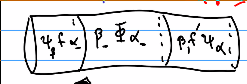
\includegraphics[width=0.8\linewidth]{mcyl}
        \caption{Picture of $\Phi_i$}%
        \label{fig:}
    \end{figure}
    Here, $\psi_{\alpha_-}$ is a homotopy from $\alpha \alpha_-$ to $\mr{id}_{X'}$ and $\psi_{\beta}$ is defined analogously. Then the three components are first $\beta_- f' \psi_{\alpha_-}$, then $\beta_- \Phi \alpha_-$, and finally $\psi_{\beta} f \alpha_-$.

    Finally, it is easy to check that the piecewise homotopies agree at the boundaries.
\end{proof}

\begin{rmk}
    This is \textbf{not} a true inverse! However, they are homotopic.
\end{rmk}

The mapping cylinder generalizes to a \textit{double mapping cylinder} $Z(f,g)$ for spans $B \xleftarrow{g} A \xrightarrow{f} C$. 

\begin{lem}
    If the diagram
    \begin{equation}
    \begin{tikzcd}
        A \arrow{r}{f} \arrow{d}{g} & B \arrow{d} \\
        C \arrow{r} & X
    \end{tikzcd}
    \end{equation}
    homotopy commutes, then we can fit the mapping cylinder $Z(f,g)$ into the diagram with an arrow $Z(f,g) \to X$. However, this arrow depends on the choice of homotopy.
\end{lem}

\begin{defn}
    $X$ is a \textit{homotopy pushout}  of the diagram in the previous lemma if $Z(f,g) \to X$ is a homotopy equivalence.
\end{defn}

Note this is \textbf{not} unique in $\ms{Top}$, but is unique in $\ms{hTop}$.

\begin{exm}
    Consider the projections $X \gets X \times Y \to Y$. Then a homotopy pushout is the join $X * Y$.
\end{exm}

\begin{exm}
    The homotopy pushout of $* \gets X \to *$ is the \textit{unreduced suspension} $\Sigma' X$. 
\end{exm}

Then recall the reduced suspension $\Sigma X = \Sigma' X / * \times I$. Then this is related to another familiar construction. The key fact is
\[ F^0(\Sigma X, Y) = \{ \gamma: X \times I \to Y \mid \gamma(x,t) = g \text{for all $t$}, \gamma(x,0) = \gamma(x,1) = y = F^0(X, \Omega Y). \]
This tells us that the suspension and loop space functors are adjoint.
Also note that concatenation makes $\Omega Y$ into an \textit{H-space} , which is a monoid in $\ms{hTop}^0$. 

Concretely, concatenation is \textit{homotopy associative} and $y \in Y$ is a (pointed) homotopy unit. Therefore, $[X, \Omega Y]$ is a group. To see this from the point of $[\Sigma X, Y]$, we see that $\Sigma X$ is a \textit{comonoid}. The map $\Sigma X \to \Sigma X \vee \Sigma X$ is simply given by collapsing $X \times \{ 1/2 \}$.  

Consider the diagram
\begin{equation}
\begin{tikzcd}
    X \arrow{r}{f} \arrow{d} & Y \arrow{d} \\
    * \arrow{r} & Y/X.
\end{tikzcd}
\end{equation}
Then we have a series of maps $F^0(Y/X,B) \to F^0(Y,B) \to F^0(X,B)$. Then define $C(f) = Z(f) / X \times \{0 \} \cup \{x\} \times I$. We now have a map $X \xrightarrow{f} Y \to C(f)$. We will use the mapping cone to replace the quotient.

\begin{lem}
    The sequence $[C(f),B]^0 \to [Y,B]^0 \xrightarrow{f} [X,B]^0$ is exact at $[Y,B]^0$ for any based space $B$. In other words, the composition sends $[C(f),B]$ to the constant map $X \to B$.
\end{lem}

\begin{proof}
    Given a map $Y \to B$ and a homotopy $\Phi$, construct $C(f) \to B$ by using the construction for the double mapping cylinder.
\end{proof}

Now we can extend to the left by considering the map $C(f) \to \Sigma X$ given by collapsing $Y$. This gives us a diagram
\[ X \xrightarrow{f} ^ \to C(f) \to \Sigma X \xrightarrow{\Sigma f} \Sigma Y \to C(\Sigma f) \to \cdots \]
Finally, we only need to check that $Y \to C(f) \to \Sigma X$ and $C(f) \to \Sigma X \to \Sigma Y$ are coexact. To check this, note that $\Sigma X$ is homotopy equivalent to $C(Y \hookrightarrow C(f))$ and the other one is easy.

\begin{cor}
    For each space $B$, we have an exact sequence
    \[ \cdots \to [\Sigma C(f),B]^0 \to [\Sigma Y, B]^0 \to [\Sigma X,B]^0 \to [C(f),B]^0 \to [Y,B]^0 \to [X,B]^0. \]
    If we extend to the left, we obtain \textit{abelian groups} because the double loop space is a commutative H-space. 
\end{cor}

\section{Homotopy Pullbacks}%
\label{sec:homotopy_pullbacks}

Now we will dualize everything and look for
\[ [B,X]^0 \to [B,Y]^0 \to [B,?]^0 \to \cdots \]
The cone is a homotopy pushout, so we will define an analogous homotopy pullback for
\begin{equation}
\begin{tikzcd}
    & * \arrow{d} \\
    x \arrow{r} & Y.
\end{tikzcd}
\end{equation}
This will be known as the \textit{homotopy fiber}. In the usual category of $\ms{Top}$, this is the actual fiber. To do this, we will replace the point by $F Y = \{ \gamma: I \to Y \mid \gamma(0) = y \}$. This is contractible by retracting every path to $y$, so we will define $F(f)$ to be the pullback of the above diagram.

\begin{lem}
    The sequence $[B,F(f)]^0 \to [B,X]^0 \to [B,Y]^0$ is exact.
\end{lem}

Proof is given by using the interval direction to construct the map from $B$ to $F(f)$. In more words, we interpret a homotopy $B \times I \to Y$ as a map $B \to FY$. In addition, this lemma constructs a fiber sequence
\[ \cdots \to \Omega F(f) \to \Omega X \to \Omega Y \to F(f) \to X \to Y, \]
which yields a long exact sequence
\[ \cdots \to [B, \Omega Y]^0 \to [B,F(f)]^0 \to [B,X]^0 \to [B,Y]^0. \]

\section{Fibrations and Cofibrations}%
\label{sec:fibrations_and_cofibrations}

Assume that $X$ is Hausdorff. 

\begin{defn}
    A map $ A \xrightarrow{i} X$ is a \textit{cofibration} if any diagram
    \begin{equation}
    \begin{tikzcd}
        A \arrow{r} \arrow{d}{i} & Y^I \arrow{d}{e_0} \\
        X \arrow{r} \arrow[dashrightarrow]{ur} & Y
    \end{tikzcd}
    \end{equation}
    admits a lift. This is called the \textit{homotopy extension property}. 
\end{defn}

In other words, we can extend diagrams of the form
\begin{equation}
\begin{tikzcd}
    A \arrow{rr}{a \times \{0\}} \arrow{dd}{i} & & A \times I \arrow{dd} \arrow{dl} \\
                                               & Y & \\
    X \arrow{rr} \arrow{ur} & & X \times I. \arrow[dashrightarrow]{ul}
\end{tikzcd}
\end{equation}

\begin{prop}
    Pushouts preserve cofibrations. In other words, for a pushout
    \begin{equation}
    \begin{tikzcd}
        A \arrow{r}{f} \arrow{d}{j} & B \arrow{d}{J} \\
        X \arrow{r} & Y,
    \end{tikzcd}
    \end{equation}
    if $j$ is a cofibration, then so is $J$.
\end{prop}

\begin{proof}
    We will diagram chase. We construct the full diagram
    \begin{equation}
    \begin{tikzcd}
        A \arrow{rrrr} \arrow{dddd}{j} \arrow{dr} & & & & A \times I \arrow{dl} \arrow{dddd} \\
        & B \arrow{rr} \arrow{dd}{J} & & B \times I \arrow{dl} \arrow{dd} \\
        & & Z \\
        & Y \arrow{rr} \arrow{ur} & & Y \times I \arrow[dashrightarrow]{ul} \\
        X \arrow{ur} \arrow{rrrr} & & & & X \times I. \arrow{ul}
    \end{tikzcd}
    \end{equation}
    Then the map $X \times I \to Z$ exists by cofibrations, and then the arrow $Y \times I \to Z$ exists because $Y \times I$ is a pushout.
\end{proof}

This proof is completely formal, and we had no idea what is going on.

\begin{exm}
    $ \{ 0 \} \subset I$ is a cofibration. To see this, note that we can identify $I$ with two sides of the square, and the retract the square onto the two sides of the interval. Note that two sides of the square form the mapping cylinder of $0 \in I$.
\end{exm}

\begin{prop}
    $A \subset X$ is a cofibration if and only if it satisfies the homotopy extension property for $Z(i)$.
\end{prop}

\begin{proof}
    Suppose the lift $X \to Z(i)^I$ exists. Then this induces a map $Z(i) \to Y$. Then we can map $X \times I \to Z(i)$ and compose.
\end{proof}

\begin{prop}
    $A \subset X$ is a cofibration if and only if it is a neighborhood deformation retract. This is defined by $\nu \colon X \to I$ and $\psi \colon X \times I \to X$ wuch that
    \begin{enumerate}
        \item $\nu^{-1}(0) = A$.
        \item $\psi(a,t) = a$ for all $a \in A, t \in I$.
        \item If $\nu(x) < 1$, then $\psi(x,1) \in A$.
        \item $\psi(x,0) = x$.
    \end{enumerate}
\end{prop}

The proof uses the previous criterion. The point is to deformation retract $X \times I$ onto $Z(i)$.

We want to be able to compute things, and we will start with cofibrant replacements. Because $\{ 0 \} \subset I$ is a cofibration, so is $X \to Z(f)$ for any $f \colon X \to Y$. Then inclusion $Y \hookrightarrow Z(f)$ is a homotopy equivalence, so we can factor $f$ into a homotopy equivalence and a cofibration. Functoriality of the mapping cylinder was discussed previously.

\begin{quest}
    Let $f \colon X \to Y$ be a homotopy equivalence such that $X,Y$ are equipped with extra structure. Can the homotopy equivalence be made compatible with this extra structure?
\end{quest}

\begin{exm}
    Suppose $X,Y$ live under a space $K$. Then we can define a homotopy equivalence under $K$.
\end{exm}

\begin{prop}
    If $i \colon K \to X,j \colon K \to Y$ are cofibrations, then $f \colon X \to Y$ is a homotopy equivalence in $\ms{Top}$ if and only if it is a homotopy equivalence in $\ms{Top}^K$.
\end{prop}

\begin{proof}
    Let $g$ denote the homotopy inverse of $f$. Then consider the space $(X, g \circ j)$ under $K$. If we fix a homotopy $gf \sim \mr{id}$, this induces an isomorphism $\varphi^{\sharp} \colon [(X,i), (X,gfi)]^K \to [(X,i), (X,i)]^K$. This is done by extending to $X \times I \to K$ by the homotopy extension property.

Note that $\varphi^{\sharp}$ is a transport map. If $i \colon A \to X$ is a cofibration and $\varphi \colon A \times I \to Y$ is a homotopy. 
\end{proof}

\begin{prop}
    Let $A \xrightarrow{i} X$ and $B \xrightarrow{j} Y$ be cofibrations. Then if $f \colon A \to B$ and $F \colon X \to Y$ make the diagram commute, then $(f, F)$ is a homotopy equivalence of pairs if and only if $f$ and $F$ are both homotopy equivalences.
\end{prop}

If we dualize everything, we replace $Y^I$ by $X \times I$. Now we consider a map $p \colon E \to B$.

\begin{defn}
    A map $p \colon E \to B$ is a \textit{Hurewicz fibration} if all diagrams of the form
    \begin{equation}
    \begin{tikzcd}
        X \arrow{r} \arrow{d} & E \arrow{d}{p} \\
        X \times I \arrow{r} \arrow[dashrightarrow]{ur} & B
    \end{tikzcd}
    \end{equation}
    admit a lift. This is called the \textit{homotopy lifting property}.  
\end{defn}

\begin{defn}
    A map $p \colon E \to B$ is a \textit{Serre fibration} if it satisfies the homotopy lifting property for all cubes. 
\end{defn}

\begin{lem}
    Pullbacks preserve fibrations.
\end{lem}

The test object we will use to study fibrations is the pullback $W(p) = \{ (e,w) \mid p(e) = w(0) \} \subset E \times B^I$.

\begin{prop}
    $W(p) \to E$ is a hommotopy equivalence. In addition, $p$ is a fibration if and only if it has the homotopy lifting property for $W(p)$.
\end{prop}

Now, let $X \xrightarrow{f} Y$ be an arbitrary map. Then we can factor $X \to W(f) \to Y$ as a fibration and a homotopy equivalence.

\begin{exm}
    All covering maps are fibrations. Also, if $A \to X$ is a cofibration, the dual $B^X \to B^A$ is a fibration. Similarly, if $E \to B$ is a fibration, then so is $Z^E \to Z^B$.
\end{exm}

Now suppose $f \colon X \to Y$ is a homotopy equivalence of spaces over $B$. Then if $p \colon X \to B$ and $q \colon Y \to B$ are fibrations, $f$ is a homotopy equivalence in $\ms{Top}$ if and only if it is a homotopy equivalence in $\ms{Top}_B$.

\section{Homotopy Groups}%
\label{sec:homotopy_groups}

Let $X$ be a based space.

\begin{defn}
    The $n$-th \textit{homotopy group}  of $X$ is 
    \[ \pi_n(X,*) = [(I^n, \partial I^n), (X,*)] \cong [I^n / \partial I^n, X]^0. \]
\end{defn}

\begin{defn}
    Given a pair $(X,A)$ of based spaces, the $n$-th \textit{relative homotopy group} is
    \[ \pi_{n+1}(X,A,*) = [(I^n, \partial I^{n+1}, \mc{J}^n), (X, A, *)] \]
    where $\mc{J}^n = \partial I^n \times I \cup I^n \times \{0 \}$. Here, the source triple is homotopy equivalent to $(D^{n+1}, S^n, *)$.
\end{defn}

We will attempt to develop some tools to compute homotopy groups. Let $F(X,A) = \qty{w \colon I \to X \mid w(0) = *, w(1) \in A}$. By splitting $(F(I^{n+1}, \partial I^{n+1}, \mc{J}), (x, A, *)) \cong F((I^n, *), (F(X,A), *))$ and using the suspension-loop adjunction, we obtain
\[ \pi_n(X, *) \cong \pi_{n-1}(\Omega X, *) \cong \cdots \cong \pi_1(\Omega^n X, *). \]
Therefore the relative homotopy group is the set of components of the $n$-th loop space of $F(X,A)$. The loop space appears in the fiber exact sequence, and $F(X,A)$ is simply the homotopy fiber of $A \to X$, so if we set $B = S^0$, we obtain from the long exact sequence
\[ \cdots \to \Omega(F(X,A)) \to \Omega A \to \Omega X \to F(X,A) \to A \to X \]
the exact sequence of homotopy groups
\[ \cdots \to \pi_0(\Omega F(X,A)) \to \pi_0 \Omega A \to \pi_0 \Omega X \to \pi_0(F(X,A)) \to \pi_0(A) \to \pi_0(X) \]
which becomes
\[ \cdots \to \pi_2(X,A) \to \pi_1(A) \to \pi_1(X) \to \pi_1(X,A) \to \pi_0(A) \to \pi_0(X). \]
\begin{warn}
    The relative homotopy group is \textbf{not} the same as the homotopy group of the quotient. 
\end{warn}

Here, we were very sloppy with basepoints and all of our homotopy groups should have carried basepoints. Last time, we showed that a homotopy $K \times I \xrightarrow{\varphi} X$ induces a transport map
\[ (A, i), (X, \varphi_0)^K \to [(A,i), (X, \varphi_1)]^k \]
if $K \to A$ is a cofibration. Applying this to $K = \mr{pt}, A = S^n$, we obtain a transport $\pi_n(X, *) \to \pi_n(X, *')$.

\begin{prop}
    The assignment $* \to \pi_n(X, *)$ defines a functor $\Pi X \to \ms{Set}$. If $n \geq 1$, the target of the functor can be replaced with $\ms{Grp}$.
\end{prop}

\begin{cor}
    \begin{enumerate}
        \item Up to some isomorphism, the $n$-th homotopy group is invariant of the choice of basepoint. The choice is not canonical unless $\pi_1$ acts trivially.
        \item If $f \colon X \to Y$ is a homotopy equivalence, then the induced map on homotopy groups is an isomorphism.
        \item $\pi_1(X,*)$ acts naturally on $\pi_n(X,*)$.
    \end{enumerate}
\end{cor}

Now suppose $E \xrightarrow{\pi} B$ is a fibration. Then the homotopy fiber is homotopy equivalent to the actual fiber $F$, so the relative homotopy groups of $F$ in $E$ are isomorphic to the homotopy groups of the base. To construct an explicit map $\pi_k(E,F,*) \gets \pi_j(B,*)$, we begin with a sphere in $B$. Then we use the homotopy lifting property to obtain a disc in $E$ with boundary in $E$.

It is easy to see the following:
\begin{enumerate}
    \item If $X$ is contractible, then $\pi_i(X,*) = 0$ for all $i > 0$.
    \item The argument we gave for $\pi_1(S^n, *)$ for $n \geq 2$ also shows that $\pi_1(S^n, *) = 0$ for $i < n$. To see this, consider $S^i \xrightarrow{f} S^n = \R^n \cup \infty$. First, we can find a homotopic map $f'$ which is smooth and transverse to $\infty$. This implies the image lies in $\R^n$ if $i < n$, so $f'$ is nullhomotopic because $\R^n$ is contractible.
    \item If $\wt{X} \to X$ is a covering map, then $\pi_i(\wt{X}, \wt{x}) \to \pi_i(X,x)$ is an isomorphism for $i > 2$. To see this, we use the lifting property for maps
        \begin{equation*}
        \begin{tikzcd}
            & \wt{X} \arrow{d} \\
            S^n \arrow{r} \arrow[dashrightarrow]{ur} & X
        \end{tikzcd}
        \end{equation*}
        because $0 = \pi_1(S^n) \to \pi_1(X)$. 

        As an example, this allows us to compute $\pi_1(S^1) = \Z$, and $\pi_i(S^1) = 0$ for $i > 1$ because the universal cover $\R$ is contractible.
    \item Consider the Hopf fibration $S^1 \to S^3 \to S^2$. Applying the long exact sequence, we have
        \[ 0 = \pi_2(S^3) \to \pi_2(S^2) \to \pi_1(S^1) \to \pi_1(S^3) = 0 \]
        and observe that $\pi_2(S^2) = \Z$.
\end{enumerate}

We would naively expect that $\pi_i(S^n) = 0$ for $i > n$, but this is incorrect. However, it is true that $\pi_n(S^n) = \Z$. For higher homotopy groups, it is easy to see that an analog of the Seifert-van Kampen theorem does not hold. If we write $S^2 = D^2 \cup D^2$, then $D^2$ and $S^1$ both have trivial $\pi_2$, but $S^2$ does not.

What does hold is Blakers-Massey. Assume that $Y = Y_1 \cup Y_2$, where the $Y_i$ are open. Suppose that $Y_0 = Y_1 \cap Y_2$ is nonempty. Then we have a map
    \[ \pi_1(Y_2, Y_0) \to \pi_i(Y, Y_1) \]
    called the \textit{excision}. 

\begin{thm}
    Assume that $(Y_1, Y_0)$ is $p$-connected and $(Y_2, Y_0)$ is $q$-connected. Then excision is an isomorphism in degree $i < p+q$ and surjective in degree $i = p+q$. This means that excision is $(p+q)$-connected as a map of pairs.
\end{thm}

Note that a pair $(X,A)$ is $p$-connected if $\pi_1(X,A,*) = 0$ for $0 \leq i \leq p$. This is equivalent to $\pi_i(A) \simeq \pi_i(X)$ for $i < p$ and $\pi_p(A) \twoheadrightarrow \pi_p(X)$.

Now we can prove that $\pi_n(S^n) = \Z$. First consider $n = 2$. Then we have a long exact sequence
\[ \cdots \to \pi_2(D^2, S^1) \to \pi_1(S^1) \to \pi_1(D^2) \to \cdots \]
and we see that $\pi_2(D^2, S^1) \cong \Z$. We now apply excision for $\pi_2(D^2_-, S^1) \to \pi_2(S^2, D^2_+) \cong \pi^2(S^2) \cong \Z$. To see that excision is an isomorphism, use the Hopf fibration.

In the next dimension, we use the same computation to see that $\pi_3(D^3, S^2) \cong \Z$ and the pairs $(D^3_+, S^2), (D^3_-, S^2)$ are $2$-connected. Then the map $(D^3_+, S^2) \to (S^3, D^3_-)$ is $4$-connected, so $\pi_3(S^3) \cong \pi_3(S^3, D^3_-) \cong \pi_3(D^3, S^2) \cong \Z$.









\end{document}
